% 与英文图源共用 v4 设计稿；生成图像与运动示意不作为试验证据。
\begin{center}
\vspace{-6pt}
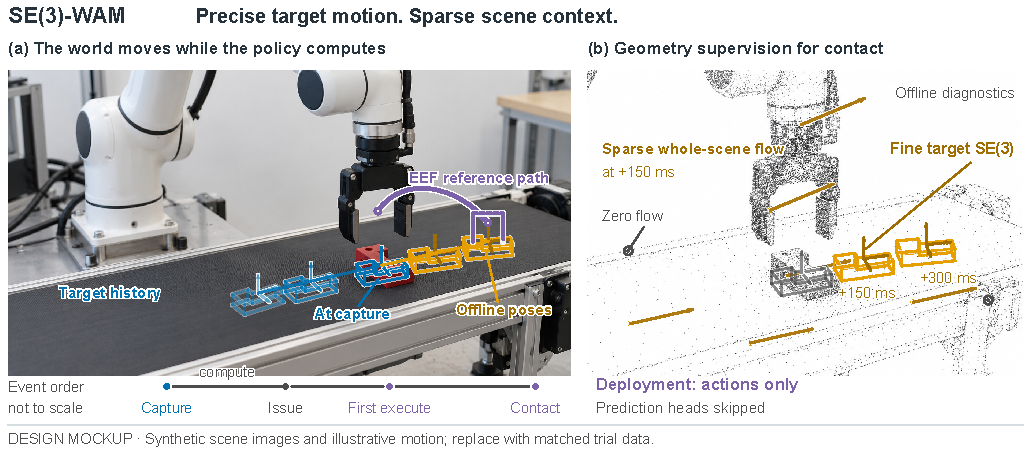
\includegraphics[width=\textwidth]{figures/Fig1/fig1_storyboard.pdf}
\captionof{figure}{\textbf{面向动态接触的几何学习。}
(a) 目标历史位姿（蓝）、未来位姿示意（橙）和末端参考路径（紫）展示观测至接触期间的运动。采集、动作发出、首次执行和接触是不同事件；事件条不按时间比例绘制。
(b) 精细目标 SE(3) 与全场景稀疏 3D 流提供训练监督。预测时域相对于采集时刻，流展示 $+150$\,ms 的位移，带圆环的点表示静态环境中的零流采样。背景点仅表示场景，不是监督网格。部署时跳过预测头，解码几何不输入动作分支。
\emph{设计示意：两幅场景图均为生成的采集状态背景；位姿、运动和接触均为示意，不是试验数据或模型输出。}}
\label{fig:teaser}
\vspace{4pt}
\end{center}
